\chapter{Hauptteil}
\section{Kraftfahrzeuge}
Das deutsche Straßenverkehrsgesetz beschreibt Kraftfahrzeuge als Landfahrzeuge, die durch Maschinenkraft bewegt werden, aber nicht an Bahngleise gebunden sind.
\footnote{Straßenverkehrsgesetz, § 1 Abs. 2}



Da Kraftfahrzeuge Landfahrzeuge sind gehören Flugzeuge, Schiffe oder Boote nicht zu der Kategorie, obwohl sie durch Maschinenkraft bewegt werden.
Auch Züge oder Trambahnen gehören nicht in in die Kategorien, da sie an Bahngleise gebunden sind.

\subsection{Teilsysteme von Kraftfahrzeugen}
Moderne Kraftfahrzeuge werden aus folgenden Teilsysteme gebildet:
\begin{itemize}
	\item Antriebseinheit
	\item Energieübertragungseinheit
	\item Stütz- und Trageeinheit
	\item Steuerungs- und Regelungseinheit
	\item Arbeitseinheit
\end{itemize}


\begin{figure}[!ht]
	\caption{Teilsysteme des Kraftfahrzeugs}
	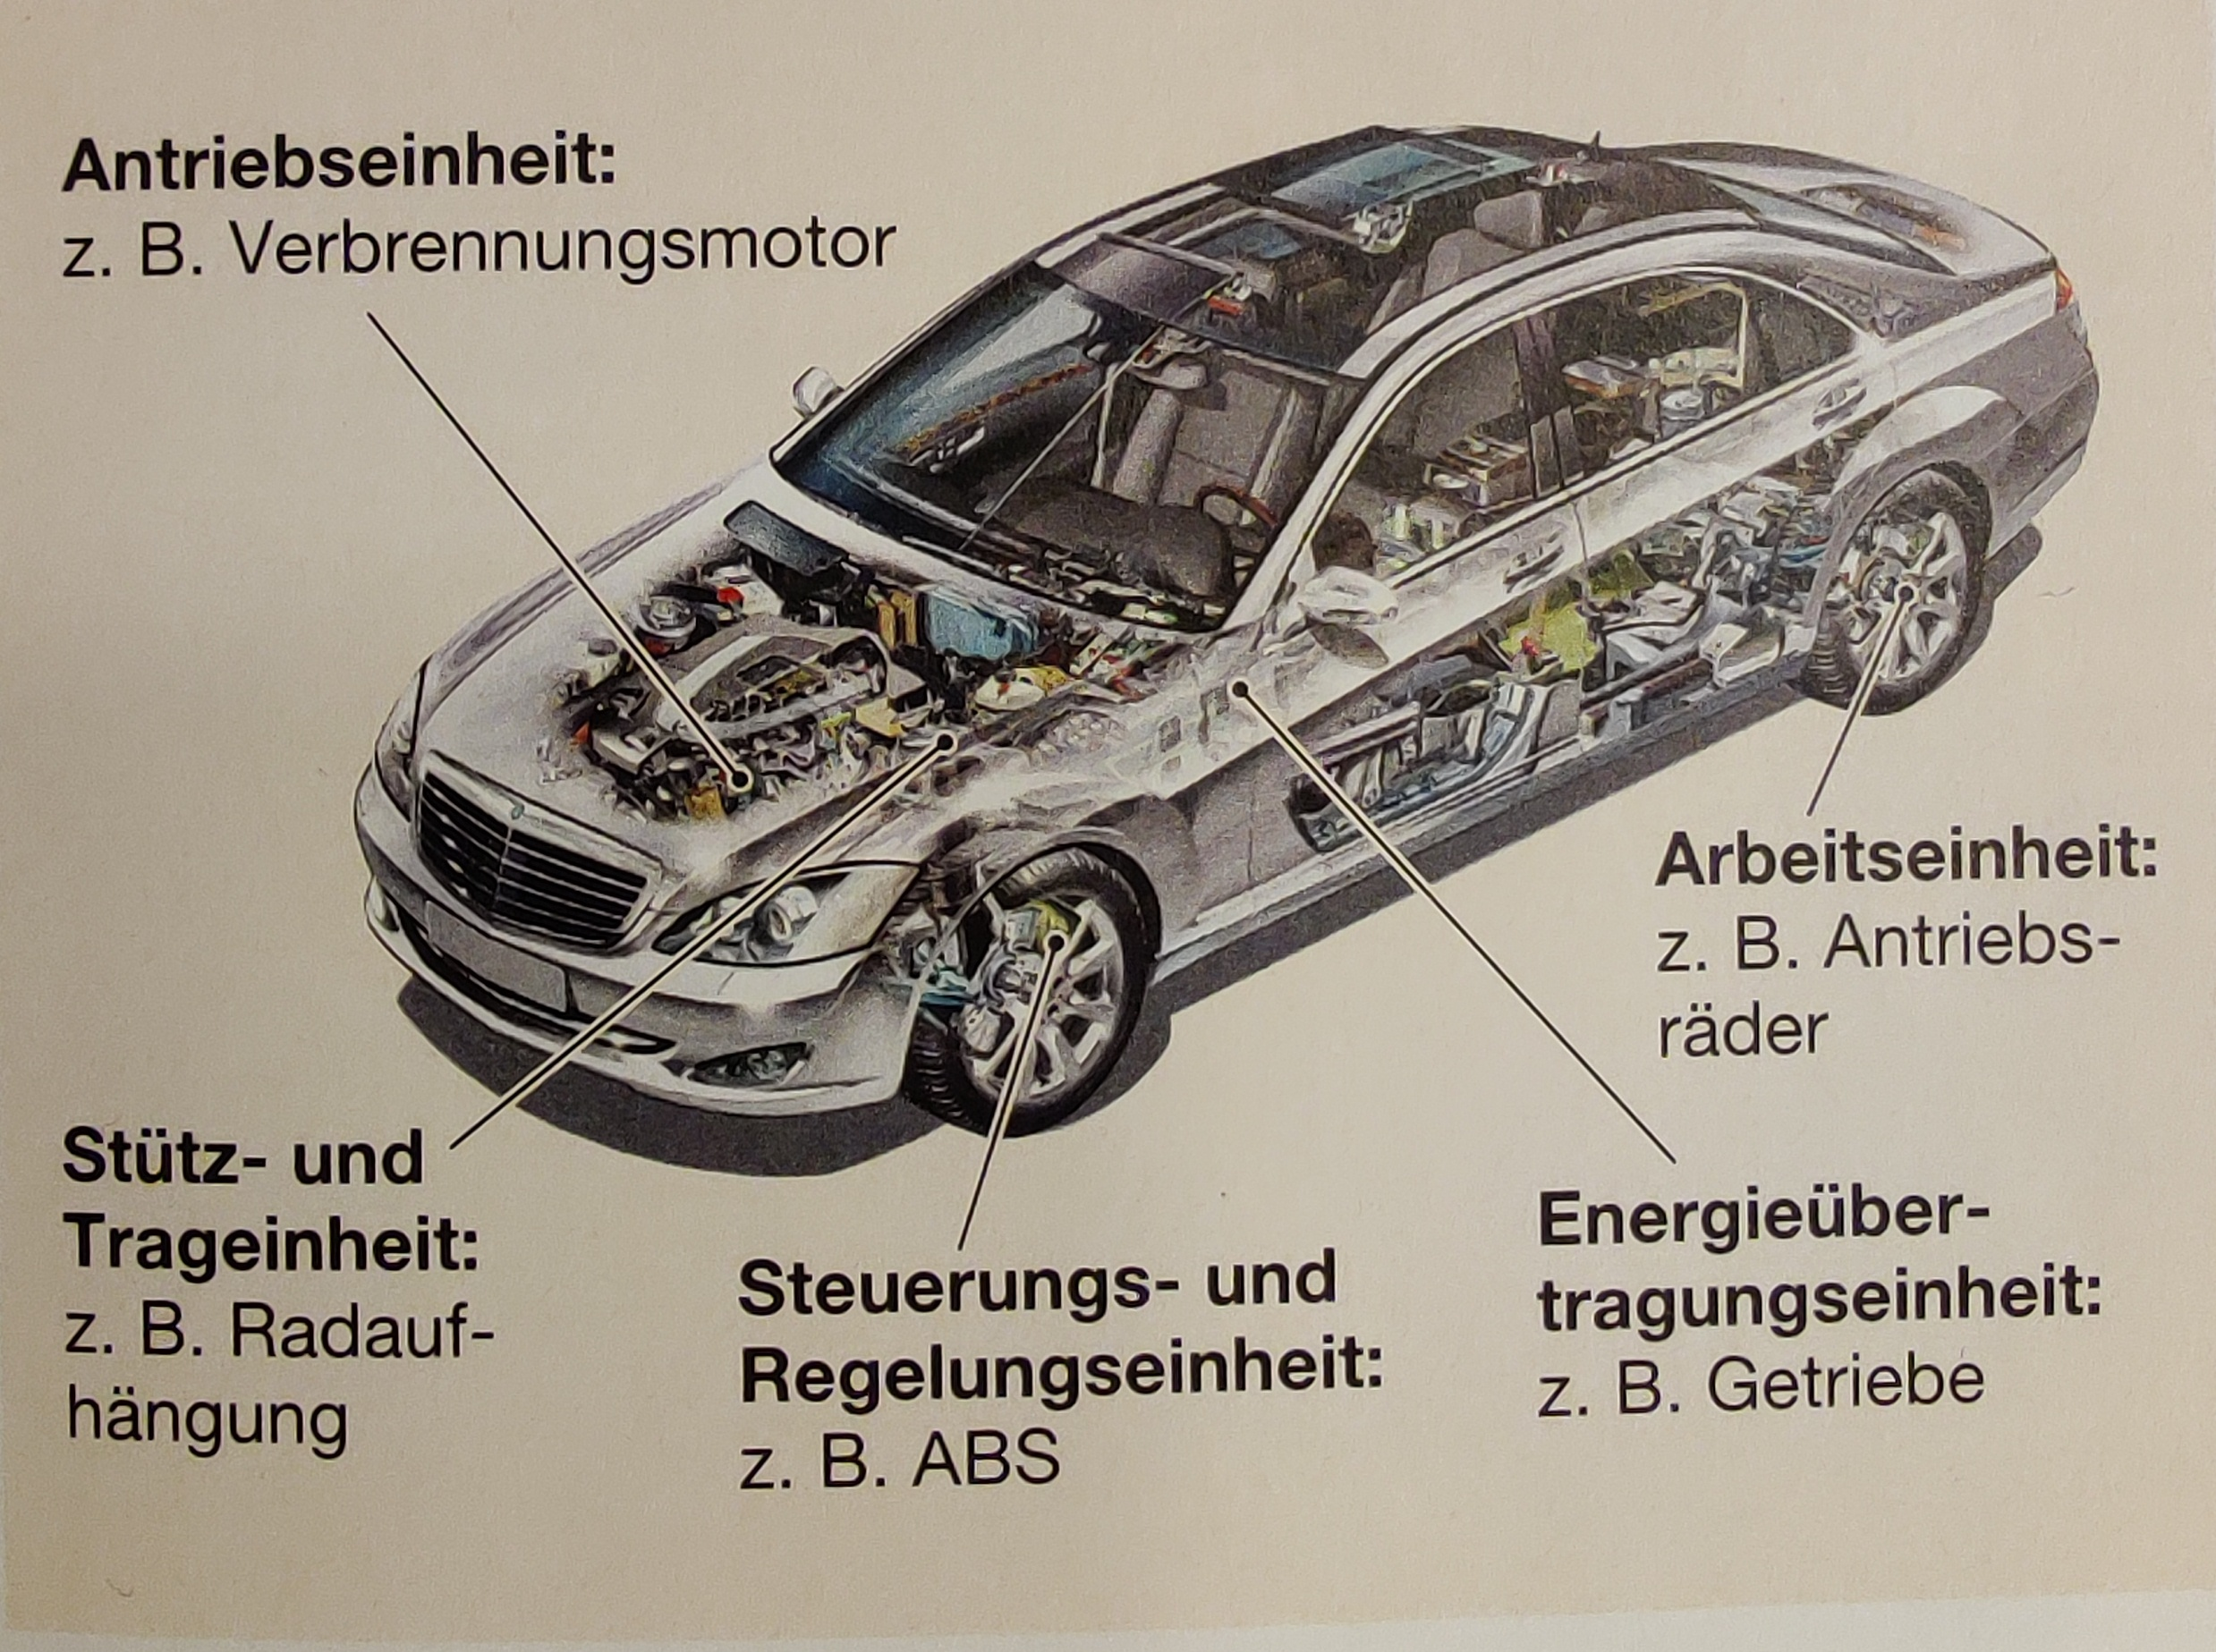
\includegraphics[scale=0.1]{assets/figures/Teilsysteme des Kraftfahrzeugs.jpg}
	\begin{flushleft}
		Quelle: Westermann S. 19
	\end{flushleft}
	\label{fig:birds}
\end{figure}


\subsubsection{Antriebseinheit}
Die Antriebseinheit wandelt die zugeführte Energie in die erforderliche Antriebsenergie um.
Diese Umwandlung wird im Motor durchgeführt.
Hauptsächlich werden Elektro- und Verbrennungsmotoren eingesetzt.

Verbrennungsmotoren unterscheiden sich von Elektromotoren durch ihre Energieerzeugung.
Die Energieerzeugung wird durch die Verbrennung von Kraftstoff erzeugt.
Dazu wird ein Kraftstoff-Luft-Gemisch in einem Brennraum mit Kolben zur Verbrennung verwendet.
Durch die Verbrennung steigt der Druck im Brennraum stark an und bewegt einen Kolben.

\subsubsection{Arbeitseinheit}
Die Arbeitseinheit ist die Verbindung zwischen den Antriebsrädern und der Fahrbahn.
Durch die Bewegung der Antriebsrädern wird das Kraftfahrzeug in Bewegung gesetzt.

\subsubsection{Energieübertragungseinheit}
Die Energieübertragungseinheit leitet die Energie in der geforderten Bewegungsart und Bewegungsgeschwindigkeit zu der Arbeitseinheit weiter.

Energieübertragungseinheiten sind Baugruppen einer Maschine, die zur Übertragung von Energie benötigt werden.
Beispiel hierfür sind Kabel die elektrische Energie leiten oder Wellen, Zahnräder und Riemen die mechanisches Drehmoment übertragen.

\subsubsection{Stütz- und Trageeinheit}
Der Rahmen oder der selbsttragende Aufbau eines Kraftfahrzeuges ist die Stütz- und Trageeinheit.
Diese haben hauptsächlich die Aufgabe, die Teilsysteme aufzunehmen und zu einer Einheit zu verbinden.

\subsubsection{Steuerungs- und Regelungseinheit}
Die Steuerungs- und Regelungseinheit beeinflusst die Stoff- und Energieumsetzung durch Informationsverarbeitung.

\subsubsection{Steuerungseinheit}
Bei der Steuerungseinheit werden verschiedene Eingangsgrößen durch das System in eine oder mehrere Ausgangsgrößen verändert.
Beispiele für Steuerungen sind:
\begin{itemize}
	\item Klimaanlage: Es wird eine Solltemperatur eingestellt.
	      Die Klimaanlage kühlt konstant.
	      Die Klimaanlage kühlt solange mit dieser eingestellten Temperatur solange sie nicht verändert wird.
	      Die Umgebungstemperatur wird nicht berücksichtigt.
	\item Licht: Der Schalter wird betätigt und das Licht wird eingeschaltet.
	      Das Licht bleibt permanent eingeschaltet.
	      Das Licht geht erst aus wenn der Schalter ausgeschaltet wird.
	      Das Umgebungslicht wird nicht berücksichtigt.
\end{itemize}

\newpage

\subsubsection{Regelungseinheit}
Bei einer Regelungseinheit werden die Eingangsgrößen mit einem Sollwert verglichen und so lange angepasst bis der Sollwert erreicht wird.
Beispiele für Regelungen sind:
\begin{itemize}
	\item Klimaautomatik: es wird eine Solltemperatur eingestellt.
	      Es wird gemessen wie warm oder wie Kalt die Temperatur ist.
	      Sollte die Temperatur unter der Solltemperatur liegen, wird die Klimaautomatik auf Heizen gestellt.
	      Sollte die Temperatur über der Solltemperatur liegen, wird die Klimaautomatik auf Kühlen gestellt.
	\item Lichtautomatik: Es gibt eine Schwelle bei der das Licht eingeschaltet werden soll.
	      Es gemessen wie hell das Umgebungslicht ist.
	      Sollte das Umgebungslicht zu gering sein wie zum Beispiel im Tunnel oder bei Dämmerung wird das Licht eingeschaltet.
	      Sobald das Umgebungslicht wieder hell genug ist zum Beispiel beim verlassen des Tunnels oder bei Sonnenaufgang, wird das Licht wieder ausgeschaltet.
\end{itemize}

\subsection{Fahrzeugklassen}

Kraftfahrzeuge können Bauartbedingt in Kategorien eingeordnet werden.
Die EU Kommission hat hierfür acht Klassen definiert.\footnote{VERORDNUNG (EU) Nr. 678/2011 DER KOMMISSION
	vom 14. Juli 2011, TEIL A ABS.1 - https://eur-lex.europa.eu/eli/reg/2011/678/oj?locale=de}

\begin{itemize}
	\item Klasse L: Leichte ein- und zweispurige Kraftfahrzeuge
	\item Klasse M: Vorwiegend für die Beförderung von Fahrgästen und deren Gepäck ausgelegte und gebaute Kraftfahrzeuge
	\item Klasse N: Vorwiegend für die Beförderung von Gütern ausgelegte und gebaute Kraftfahrzeuge
	\item Klasse O: Anhänger, die sowohl für die Beförderung von Gütern und Fahrgästen als auch für die Unterbringung von Personen ausgelegt und gebaut sind
	\item Klasse S: unvollständige Fahrzeuge, die der Unterklasse der Fahrzeuge mit besonderer Zweckbestimmung zugeordnet werden soll
	\item Klasse R: Anhänger, die in der Land- und Forstwirtschaft verwendet werden
	\item Klasse S: Maschinen, die in der Land- und Forstwirtschaft zum Einsatz kommen und gezogen werden
	\item Klasse T: Zugmaschinen, die in der Land- und Forstwirtschaft verwendet werden wie Traktoren
	\item Klasse C: Zugmaschinen, die in der Land- und Forstwirtschaft verwendet werden und auf Ketten laufen wie ein Bagger
\end{itemize}

Die relevantesten Klassen sind M und N.
\vspace{0.5cm}

\subsection{Klasse M}
In der Klasse M werden Kraftfahrerzeuge eingeordnet die für die Beförderung von Personen und Gepäck zuständig sind und mindestens 4 Räder haben sowie eine Hochgeschwindigkeit von über 25 \ac{kmh} haben.
\newline
Die Klasse M spaltet sich in 3 Unterklassen auf:
\begin{itemize}
	\item {Klasse M1}
	\item {Klasse M2}
	\item {Klasse M3}
\end{itemize}
\subsubsection{Klasse M1}
Kraftfahrzeuge der Klasse M1 haben über die Eigenschaften der Klasse M noch folgende weitere Eigenschaften:
\begin{itemize}
	\item {nicht mehr als 8 Sitzplätze und 1 Platz für den Fahrer}
	\item {keine Stehplätze}
	\item {zulässiges Gesamtgewicht von maximal 3,5 \ac{t}}
\end{itemize}

In der Klasse M1 sind Kraftfahrzeuge wie Personenkraftwagen(Limousine, Cabrio) und Wohnmobile zu finden.

\subsubsection{Klasse M2}
Kraftfahrzeuge der Klasse M2 haben über die Eigenschaften der Klasse M noch folgende weitere Eigenschaften:
\begin{itemize}
	\item {mehr als 8 Sitzplätze}
	\item {zulässiges Gesamtgewicht von maximal 5 \ac{t}}
\end{itemize}

In der Klasse M2 sind Kraftfahrzeuge wie ein Eindecker-Bus bis 5 \ac{t} oder ein Doppeldecker-Bus bis 5 \ac{t} zu finden.

\subsubsection{Klasse M3}

Die dritte Unterklasse der Klasse M ist M3.

Kraftfahrzeuge der Klasse M3 haben über die Eigenschaften der Klasse M noch folgende weitere Eigenschaften:
\begin{itemize}
	\item {mehr als 8 Sitzplätze}
	\item {zulässiges Gesamtgewicht von über 5 \ac{t}}
\end{itemize}

In der Klasse M3 sind Kraftfahrzeuge wie ein Eindecker-Bus über 5 \ac{t} oder Doppeldecker-Bus über 5 \ac{t} zu finden.

\subsection{Klasse N}
In der Klasse N werden Kraftfahrerzeuge eingeordnet die für die Beförderung von Gütern zuständig sind und mindestens 3 Räder haben sowie ein zulässiges Gesamtgewicht von über 1 \ac{t} haben.
Die Klasse N spaltet sich in 3 Unterklassen auf:
\begin{itemize}
	\item {Klasse N1}
	\item {Klasse N2}
	\item {Klasse N3}
\end{itemize}

\subsubsection{Klasse N1}
Fahrzeuge zur Güterbeförderung mit einer zulässigen Gesamtmasse bis zu 3,5 \ac{t}.
In der Klasse N1 sind Kraftfahrzeuge die in dicht besiedelten Regionen gut zurecht kommen, wie Paketzusteller oder Fahrzeuge der Post.


\subsubsection{Klasse N2}
Fahrzeuge zur Güterbeförderung mit einer zulässigen Gesamtmasse von zu 3,5 \ac{t} bis 12 \ac*{t}.
In der Klasse N2 sind Kraftfahrzeuge die regional Güterbefördern, dies könnten Kraftfahrzeuge die Waren aus einem Zentrallager in die Filialen transportieren.
Diese Kraftfahrzeuge sind darauf ausgelegt hunderte Kilometer zurückzulegen.


\subsubsection{KLasse N3}
Fahrzeuge zur Güterbeförderung mit einer zulässigen Gesamtmasse von mehr als 12 \ac{t}.
In der Klasse N3 sind Kraftfahrzeuge die überregional Güterbefördern, wie ein Kraftfahrzeug das große Mengen an Ladung fassen kann und darauf ausgelegt sind tausende Kilometer zurückzulegen.

\subsection{Autonome Kraftfahrzeuge}
Beim autonomen Fahren, fährt ein Kraftfahrzeug verwaltungsgemäß selbständig.
Für Kraftfahrzeuge wurden von der \ac{SAE} Automatisierungsstufen definiert\cite{PRACTICE}.
\begin{itemize}
	\item Stufe 0 (Keine Automation)
	\item Stufe 1 (Assistenzsysteme)
	\item Stufe 2 (Teilautomatisierung)
	\item Stufe 3 (Bedingte Automatisierung)
	\item Stufe 4 (Hochautomatisierung)
	\item Stufe 5 (Vollautomatisierung)
\end{itemize}
\subsubsection{Was passiert in den Stufen?}
Die Stufen unterscheiden sich im wesentlichen nur durch die Anzahl der Automatisierungsgrade.

\vspace{0.5cm}

In der Stufe 0 (Keine Automation):
\begin{itemize}
	\item keine Assistenzsysteme
	\item Kraftfahrzeug kann keine Fahraufgaben übernehmen
	\item Fahrer kontrolliert permanent das Fahrzeug
\end{itemize}

\vspace{0.5cm}

In der Stufe 1 (Assistenzsysteme):
\begin{itemize}
	\item Assistenzsysteme wie zum Beispiel ein System zur automatischen Geschwindigkeitsregelung oder eine Berganfahrhilfe
	\item Fahrer hat eine passive Unterstützung bei Fahraufgaben
	\item Kraftfahrzeug kann keine Fahraufgaben übernehmen
	\item Fahrer kontrolliert permanent das Fahrzeug
\end{itemize}

\vspace{0.5cm}

In der Stufe 2 (Teilautomatisierung):
\begin{itemize}
	\item Assistenzsysteme, wie zum Beispiel der Spurführungsassistent oder Stauassistent
	      \begin{itemize}
		      \item automatisch bremsen
		      \item automatisch beschleunigen
		      \item automatisch lenken
	      \end{itemize}
	\item Kraftfahrzeug kann Fahraufgaben teilautomatisiert übernehmen
	\item Fahrer kann sich für kurze Zeit von den Fahraufgaben abwenden
	\item Fahrer muss jeder Zeit die teilautomatisierte Fahraufgabe übernehmen können
\end{itemize}

\vspace{0.5cm}

In der Stufe 3 (Bedingte Automatisierung):
\begin{itemize}
	\item hochautomatisierte Assistenzsysteme
	\item Kraftfahrzeug kann Fahraufgaben unter bestimmten Voraussetzungen vollständig übernehmen
	\item Fahrer kann sich unter bestimmten Voraussetzungen von den Fahraufgaben abwenden
	\item Fahrer muss innerhalb von wenigen Sekunden die Fahraufgabe übernehmen können
\end{itemize}

\vspace{0.5cm}

In der Stufe 4 (Hochautomatisierung):
\begin{itemize}
	\item hochautomatisierte Assistenzsysteme
	\item Kraftfahrzeug kann Fahraufgaben in hochkomplexen Verkehrssituationen vollständig übernehmen
	\item Fahrer kann sich von den Fahraufgaben abwenden
	\item Fahrer muss fahrtüchtig sein, um im Bedarfsfall die Fahraufgabe übernehmen zu können
\end{itemize}

\vspace{0.5cm}

In der Stufe 5 (Vollautomatisierung):
\begin{itemize}
	\item hochautomatisierte Assistenzsysteme
	\item Kraftfahrzeug übernimmt alle Fahraufgaben vollständig
	\item Fahrer ist nicht erforderlich
	\item alle Personen im Wagen werden zu Passagieren
\end{itemize}


Autonome Kraftfahrzeuge sind Kraftfahrzeuge die nicht nur automatisch fahren sondern von einem System gesteuert werden.
Somit sind diese Kraftfahrzeuge aus Sicht der Nutzenden autonom.

Während manche in der Verbreitung autonomer Kraftfahrzeuge die Lösung vieler Probleme sehen können,
vermuten andere eine Verschlechterung der Verkehrs- und Umweltlage.

Die Bedeutung von autonomen Kraftfahrzeugen hängt sowohl von der technischen Komplexität als auch von den politischen Regulierung ab.

In welchem Maß das Level 5 System im Straßenverkehr teilnimmt entscheidet vorerst der gesetzliche Rahmen.
Dies ist wiederum abhängig wie der zukünftige Verkehr aussehen soll.
\subsection{Umweltbelastungen durch Kraftfahrzeuge}
Kraftfahrzeuge belasten die Umwelt auf verschiedene Arten.
Hierunter fallen
die Erzeugung von Rohstoffen für Materialien die für die Produktion von Kraftfahrzeugen benötigt werden,
die tatsächliche Produktion von Kraftfahrzeugen,
der Betrieb von Kraftfahrzeugen,
sowie die Entsorgung von Kraftfahrzeugen.

Gerade der Betrieb von Kraftfahrzeugen belastet die Umwelt durch die verschieden Arten von Schadstoffen.
Unterschieden wird die Art der Belastung,
durch die Verbrennung entstandene Abgase,
Feinstaub der durch die Verbrennung, sowohl auch durch den Abrieb von Reifen und Bremsen freigesetzt wird
und die Infrastruktur der Straßen, Parkplätze und anderer Einrichtungen.

\subsection{Verbrennungsabgase}
Durch Verbrennung von Kraftstoffen entstehen verschied giftige Schadstoffe:
\begin{itemize}
	\item {\ac{CO}}
	\item {\ac{NO}}
	\item unverbrannte Kohlenwasserstoffe (HC)
\end{itemize}
Die Abgase strömen nach der Verbrennung im Verbrennungsraum durch die Abgasanlage in die Umwelt.
Es gibt auch ungiftige Stoffe die durch die Verbrennung abgegeben werden wie \ac{zb} \ac{Wasser} und \ac{CO2}.
Die Menge der Abgase die durch die Abgasanlage strömen ist von der Größe des Motors sowie dem Lastzustand des Motors abhängig.

\subsection{Feinstaub}
Feinstaub ist ein fester oder flüssiger Stoff der nicht sofort zu Boden sinkt.
Neben der Art des Feinstaubes ist unter anderem die Wetterlage für die Verbreitung und Absenkung von Feinstaub entscheidend.

Luftfeuchtigkeit beeinträchtigt die Ausbreitung von Feinstaub da sich dieser bei geringer Luftfeuchtigkeit länger in Luft halten kann sich besser ausbreiten kann.

Feinstäube werden als Particle Matter (PM, zu deutsch Stoffteilchen) bezeichnet. Diese Luftschadstoffe sind gesundheitsschädlich.

Unterschieden wird zwischen Feinstaub der aus natürlichen Quellen entstanden ist und Feinstaub der durch menschliches Handeln entstanden ist.

\subsubsection{Feinstaub aus natürlichen Quellen}
Natürlicher Feinstaub entsteht ohne menschliches Handeln durch:
\begin{itemize}
	\item Vulkane
	\item Wald- und Buschbrände
	\item Pollen
	\item Sporen
\end{itemize}


\subsubsection{Feinstaub durch menschliches Handeln}
Feinstaub der durch menschliches Handeln entstanden ist wird auch anthropogener Feinstaub genannt.
Feinstaub durch menschliches Handeln entsteht durch:
\begin{itemize}
	\item Verbrennung und Abrieb vom Straßenverkehr
	\item Verbrennungsabgase von Kraftwerken und Müllverbrennungsanlagen
	\item Brände von Gegenständen
	\item Industrieprozesse wie die Stahlerzeugung
\end{itemize}

Einrichtungen der Umweltzonen und Festlegung von Fahrverboten durch die Kommunen und Städte können zur Verbesserung der Luftreinhaltung führen.
Das befahren einer Umweltzone ist dann nur mit einer entsprechenden Kennzeichnung des Fahrzeuges möglich, die man bei der zuständigen Behörde erlangen kann.



\subsection{Infrastruktur}
Auch die Infrastruktur belastet die Umwelt, indem:
\begin{itemize}
	\item Wälder abgeholzt werden um die Verkehrsanbindung zu verbessern
	\item Straßen vergrößert um ein höheres Verkehrsaufkommen zu bewältigen
	\item starke Erhitzung durch Sonneneinstrahlung auf dunklen Verkehrswegen
	\item Grünflächen abgeschafft werden um mehr Parkmöglichkeiten zu gewinnen
\end{itemize}


\section{Umweltbelastung nach Bedingungen}
Die Umweltbelastung kann stark nach Betriebszuständen variieren.
So verbraucht ein Fahrzeuge das bergab fährt weniger Kraftstoff und stößt somit auch weniger Luftschadstoffe aus.
Die Umweltbelastung durch Luftschadstoffe hängt von folgendem ab:
\begin{itemize}
	\item dem Fahrverhalten des Fahrers, wie dem Beschleunigungsverhalten und der Fahrgeschwindigkeit ab
	\item der Effizienz des Fahrzeugs, je effizienter desto besser
	\item dem Gewicht des Fahrzeugs, je leichter desto weniger Gewicht muss beschleunigt und gebremst werden
	\item der Fahrstrecke, fährt das Fahrzeug eine Steigung wird mehr Kraftstoff benötigt
	\item dem Wetter, je nach Wind wird mehr oder weniger Kraftstoff benötigt
	\item dem Betriebszustand, wenn sich das Fahrzeug nicht im Betriebszustand befindet wird Energie verwendet um den Betriebszustand zu erreichen
\end{itemize}








\subsection{Aktueller Stand}
\subsection{Gesetzliche Regelungen}
Was ist bereits wo erlaubt?\\
Welche Länder haben was freigegeben?


\section{Erkenntnisse}
Hauptsächlich wird Sicherheit und die Senkung schädlicher Emissionen sowie das Erreichen der
Klimaschutzziele im Verkehr die größte Rolle spielen.


\subsection{Beschreibung der verwendeten Untersuchungsmittel}

\subsection{Diskussion der Forschungsfrage}

\subsection{Gründe für die Wahl der Hypothese}

\subsection{Darstellung und Diskussion der Erkenntnisse aus der Literatur}

\subsection{Schlussfolgerungen auf die Forschungsfrage}

\subsection{Verifikation der Hypothese}

\subsection{Praktische Konsequenzen}
